\documentclass[tikz]{standalone}

\usepackage{amsmath}
\usepackage{physics}

\usetikzlibrary{arrows.meta,positioning}

\begin{document}
	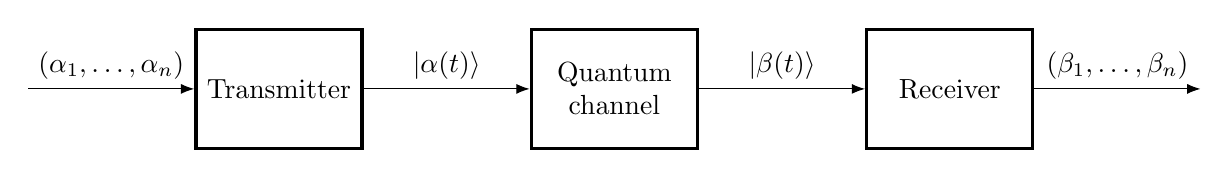
\begin{tikzpicture}[
		node distance=6em,
		block/.style={draw, very thick, minimum height=10ex, minimum width=6em, align=center},
	]
		\coordinate (in) at (0,0);
		\node (tx) [block, right=of in] {Transmitter};
		\node (ch) [block, right=of tx] {Quantum\\channel};
		\node (rx) [block, right=of ch] {Receiver};
		\coordinate[right=of rx] (out);
		
		\draw[-Latex] (in) -- node[above]{$\left(\alpha_1,\dots,\alpha_n\right)$} (tx);
		\draw[-Latex] (tx) -- node[above]{$\ket{\alpha(t)}$} (ch);
		\draw[-Latex] (ch) -- node[above]{$\ket{\beta(t)}$} (rx);
		\draw[-Latex] (rx) -- node[above]{$\left(\beta_1,\dots,\beta_n\right)$} (out);
	\end{tikzpicture}
\end{document}
